%%%%%%%%%%%%%%%%%%%%%%%

\section{Fonction moduler/commuter/traiter}\label{fonction-modulercommuter}

\hypertarget{introduction}{%
\subsection{Introduction}\label{introduction}}

Dans la chaîne fonctionnelle, le modulateur d'énergie (ou distributeur
d'énergie ou pré actionneurs) est le composant qui fait le lien entre la
chaîne d'information et la chaîne d'énergie. Ainsi, à partir d'une
faible puissance énergétique provenant de la fonction «~Traiter~» (l'API
ou la carte de commande), il peut faire transiter une grande puissance
(provenant de la fonction «~Alimenter~» ou «~Stocker~».

\begin{defi}{Définition : Tout ou rien -- Variateur}

Les distributeurs «~tout ou rien~» permettent d'envoyer toute l'énergie
de l'alimentation vers le convertisseur.

Les distributeurs de type «~variateur~» permettent de moduler l'énergie
envoyée au convertisseur. 

\end{defi}

\begin{exemple}

Un interrupteur de lumière peut être considéré comme un distributeur
tout ou rien.

Le variateur d'une lampe halogène peut être considéré comme un \ldots{}
variateur. \\
\end{exemple}

\begin{defi}{Définition : Monostable -- Bistable}

Un pré-actionneur est dit monostable s'il a besoin d'un ordre pour le
faire passer de sa position de repos à sa position de travail et que le
retour à sa position de repos s'effectue automatiquement lorsque l'ordre
disparait : \textbf{il n'est stable que dans une seule position}.

Un pré-actionneur est dit bistable s'il a besoin d'un ordre pour passer
de sa position repos à sa position travail et qu'il reste en position
travail à la disparition de cet ordre. Il ne peut revenir à sa position
repos que s'il reçoit un second ordre : \textbf{il est stable dans les
deux positions}. \\

\end{defi}

\begin{exemple}
Un interrupteur de lumière peut être considéré comme un distributeur
bistable. Il faut appuyer dessus pour allumer une lumière et appuyer une
seconde fois pour l'éteindre. \\
\end{exemple}

\subsection{Les modulateurs électriques}

\subsubsection{Le relais (ou contacteur de puissance)}

Le relais est un dispositif électrique permettant de commander un circuit
de commande ou un circuit de puissance.

Le circuit secondaire alimente la partie que l'on veut commander.
Lorsque la bobine est alimentée le levier pivote provoquant la fermeture
du contact. Certains relais peuvent aussi être actionnés manuellement.

\begin{tabular}{ccc}
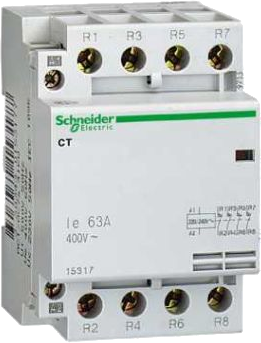
\includegraphics[width=1.21388in,height=1.59525in]{media/image95.png} &
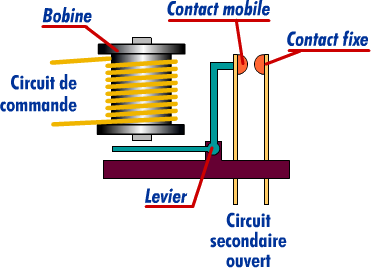
\includegraphics[width=2.34736in,height=1.69567in]{media/image96.png} &
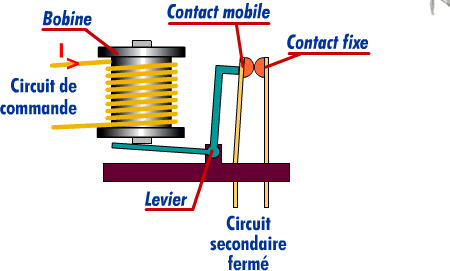
\includegraphics[width=2.4015in,height=1.7093in]{media/image97.png} \\
\end{tabular}



\textbf{Contacteur électrique monostable}

\begin{tabular}{m{.45\linewidth}m{.45\linewidth}}

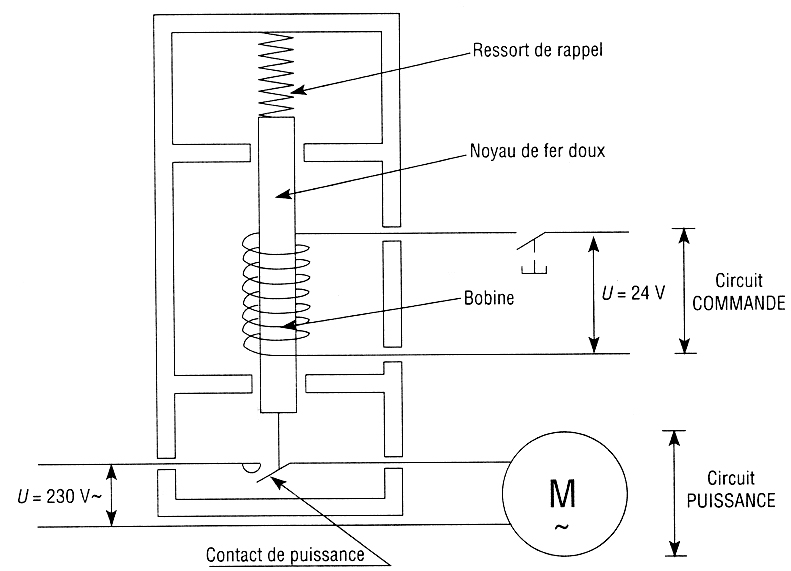
\includegraphics[width=.9\linewidth]{media/image98.png}  &

Quand la bobine reçoit un ordre de marche (appui sur
le bouton poussoir) la bobine est alimentée par un courant, créant ainsi
un champ magnétique. Le champ magnétique créé dans la bobine provoque le
déplacement du noyau de fer doux vers le haut. Le contact de puissance
est alors fermé.

Le moteur est alimenté puis mis en rotation.

Quand l'ordre de marche est interrompu (bouton relâché), le circuit de
commande est ouvert. La bobine n'est plus alimentée et le ressort de
rappel fait redescendre le noyau de fer doux.

Le circuit de puissance s'ouvre et le moteur n'est plus alimenté.

Ce contacteur est monostable car il alimente en énergie électrique le
moteur tant que l'ordre est maintenu. 

\end{tabular}

\textbf{Contacteur électrique bistable}

\begin{tabular}{m{.45\linewidth}m{.45\linewidth}}
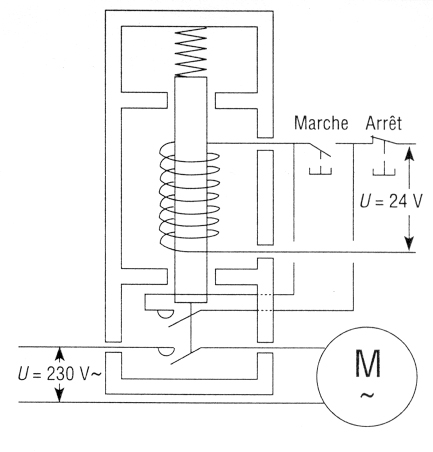
\includegraphics[width=.9\linewidth]{media/image99.jpeg}&
Ce contacteur est bistable : il faut un ordre (court) pour que le moteur
soit alimenté. Le moteur continue à être alimenté même quand l'ordre de
marche a disparu. Il faut un ordre d'arrêt (court) pour que le moteur ne
soit plus alimenté. 
\end{tabular}


\textbf{Symbolisation des contacts}
\begin{center}
\begin{tabular}{ccc}
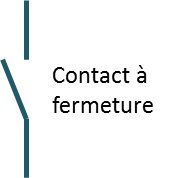
\includegraphics[width=0.79201in,height=0.7874in]{media/image100.png} &
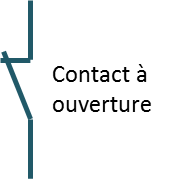
\includegraphics[width=0.76541in,height=0.7874in]{media/image101.png} &
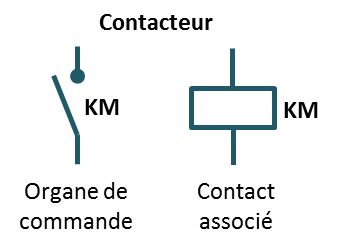
\includegraphics[width=1.36856in,height=0.98425in]{media/image102.png} \\
\end{tabular}
\end{center}


\subsubsection{Le hacheur (convertisseur statique)}

\begin{minipage}[c]{2.1in}
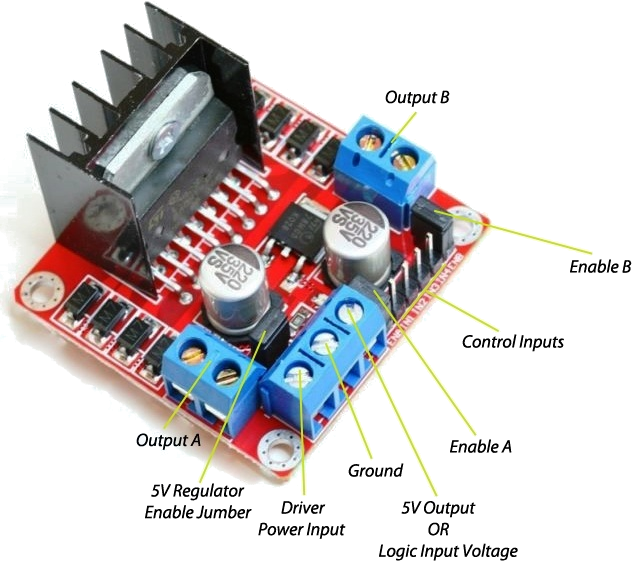
\includegraphics[width=2.0486in,height=1.82318in]{media/image103.png} 
\end{minipage}\hfill
\begin{minipage}[c]{10cm}
Lorsqu'on souhaite contrôler la fréquence de rotation d'un moteur à
courant continu ou moduler la puissance électrique s'appliquant sur une
charge, il est nécessaire de moduler sa tension d'alimentation. On
pourrait pour cela utiliser un pont diviseur, mais cette technologie
serait très énergivore à cause des pertes joules qui apparaitraient dans
les résistances. Historiquement des transistors linéaires étaient
utilisés mais ils sont couteux et peu fiables. On utilise désormais un
hacheur.
\end{minipage}

Un hacheur est composé de transistors «~tout ou rien~» utilisant la
technologie «~MOSFET~». Cette technologie permet de commuter (laisser
passer ou non) des courants importants avec une bonne fiabilité, un bon
rendement et une rapidité de commutation bien supérieure au relai. Une
bonne coordination de l'ouverture et de la fermeture de ces
interrupteurs permet de générer une tension ayant une forme de créneau
où les temps à l'état bas et à l'état haut sont réglables. 

Le hacheur est caractérisé par sa période de hachage (980 Hz pour une
carte Arduino Leonardo), ainsi que par le rapport cyclique (variable),
définit par le pourcentage de la période passé à l'état haut. Il envoie
ainsi un signal appelé MLI (Modulation de Largeur d'Impulsion) ou PWM
(Pulse Width Modulation).

\begin{tabular}{p{.3\linewidth}p{.3\linewidth}p{.3\linewidth}}
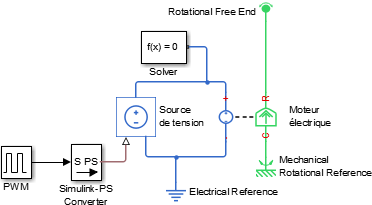
\includegraphics[width=.9\linewidth]{media/image104.png} &
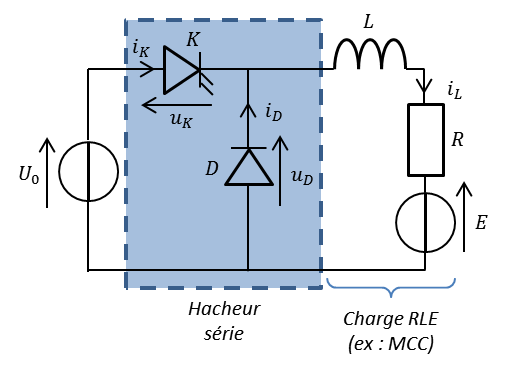
\includegraphics[width=.9\linewidth]{media/image105.png} &
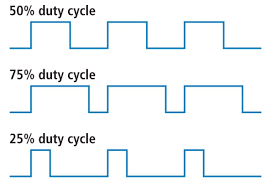
\includegraphics[width=.9\linewidth]{media/image106.png} \\
\emph{Modèle simplifié du pilotage d'un moteur électrique à courant
continu} & \emph{Schéma proche du câblage réel. L'interrupteur K est
commandé par le signal MLI} & \emph{Signal MLI avec 3 rapport cycliques
distincts} \\
\end{tabular}

Dans le cas précédent, si le moteur est alimenté par un créneau valant
24 V 25\% du temps. Il est donc alimenté en 6 V en moyenne.


\subsubsection{L'onduleur (variateur)}

Les moteurs triphasés sont physiquement alimentés par 3 fils. La tension
est sinusoïdale et décalée dans chacun d'entre eux d'un tiers de
période. Afin de générer un signal sinusoïdal de fréquence et
d'amplitude voulue on a recours à un onduleur.

Pour cela, en règle générale, on redresse la tension issue de
l'alimentation du secteur puis on régénère un signal avec l'onduleur.

\begin{tabular}{cc}
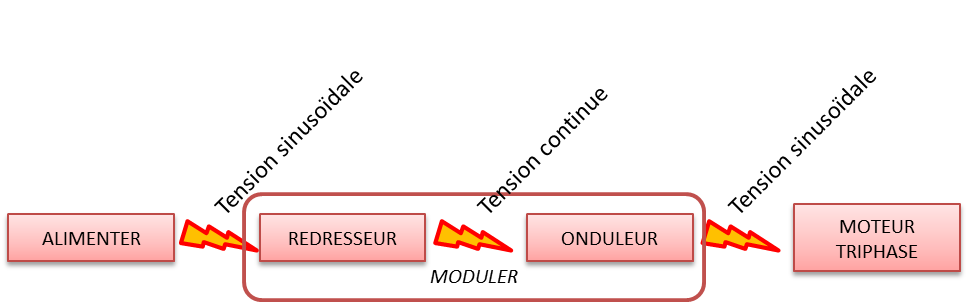
\includegraphics[width=3.95349in,height=0.98369in]{media/image107.png} &
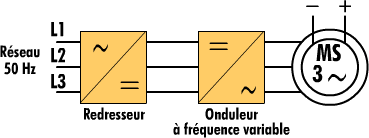
\includegraphics[width=2.39535in,height=0.89582in]{media/image108.png} \\
\end{tabular}

Le variateur est une forme d'onduleur qui permet de piloter avec
précision la vitesse ou la position d'un moteur triphasé. Pour cela il
utilise en général un capteur afin de connaitre la position du rotor et
alimenter la bonne phase. Certaines technologies peuvent déterminer la
position du rotor sans capteur en mesurant les effets d'induction dans
les phases (montée et descente de courant lorsque l'on commute la phase)
\emph{technologie sensorless}.


\subsubsection{Notion de schéma électrique}

\begin{tabular}{p{.47\linewidth}p{.47\linewidth}}
\textbf{Inversion de sens d'un moteur CC.} & \textbf{Inversion de sens
d'un moteur triphasé asynchrone} \\
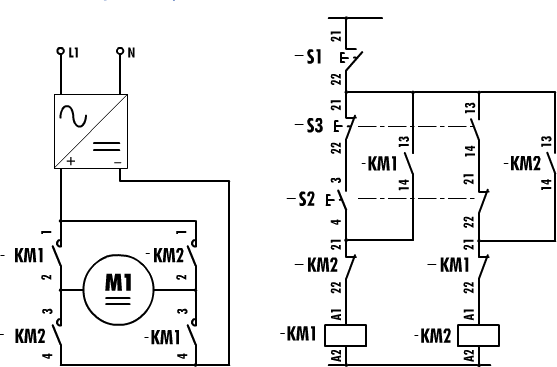
\includegraphics[width=.9\linewidth]{media/image109.png} &
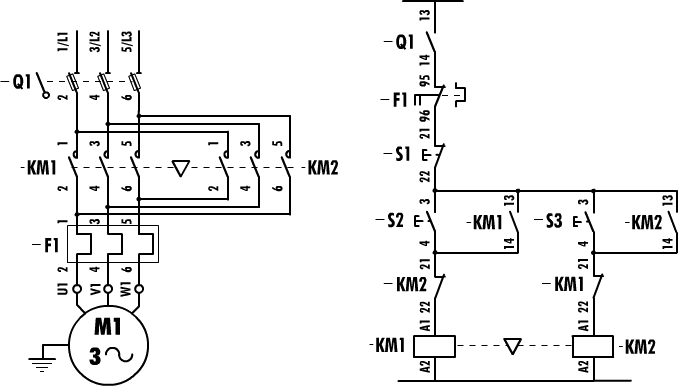
\includegraphics[width=.9\linewidth]{media/image110.png} \\
\end{tabular}

\subsection{Les modulateurs pneumatiques et hydrauliques}

\begin{defi}{Énergie hydraulique et pneumatique -- Fluides}

\textbf{Énergie pneumatique} : le fluide utilisé est de l'air comprimé.

\textbf{Énergie hydraulique} : le fluide utilisé est une huile
hydraulique minérale ou difficilement inflammable (aqueuse ou non). \\

\end{defi}


\subsection{Les distributeurs}

Les distributeurs sont les préactionneurs des vérins pneumatiques et
hydrauliques.

Ils servent d'«~aiguillages~» en dirigeant le fluide dans certaines
directions. Les plus utilisés sont les distributeurs à tiroir. 

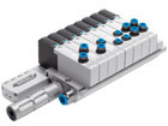
\includegraphics[width=1.81782in,height=1.36364in]{media/image111.png}

\begin{tabular}{p{.45\linewidth}p{.45\linewidth}}
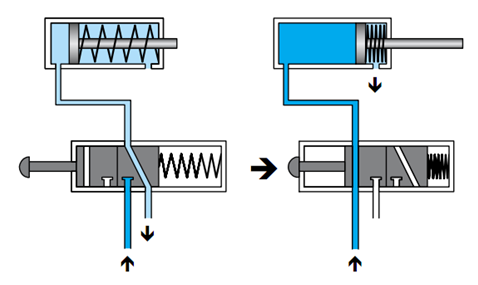
\includegraphics[width=3.14961in,height=1.88001in]{media/image112.png} & 
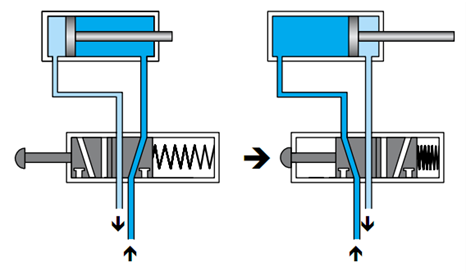
\includegraphics[width=3.14961in,height=1.85091in]{media/image113.png} \\

\emph{Vérin simple effet et distributeur 3/2 monostable NF à commande
manuelle par bouton} &
\emph{Vérin double effet et distributeur 5/2 monostable à commande
manuelle par bouton} \\
\end{tabular}


\begin{center}
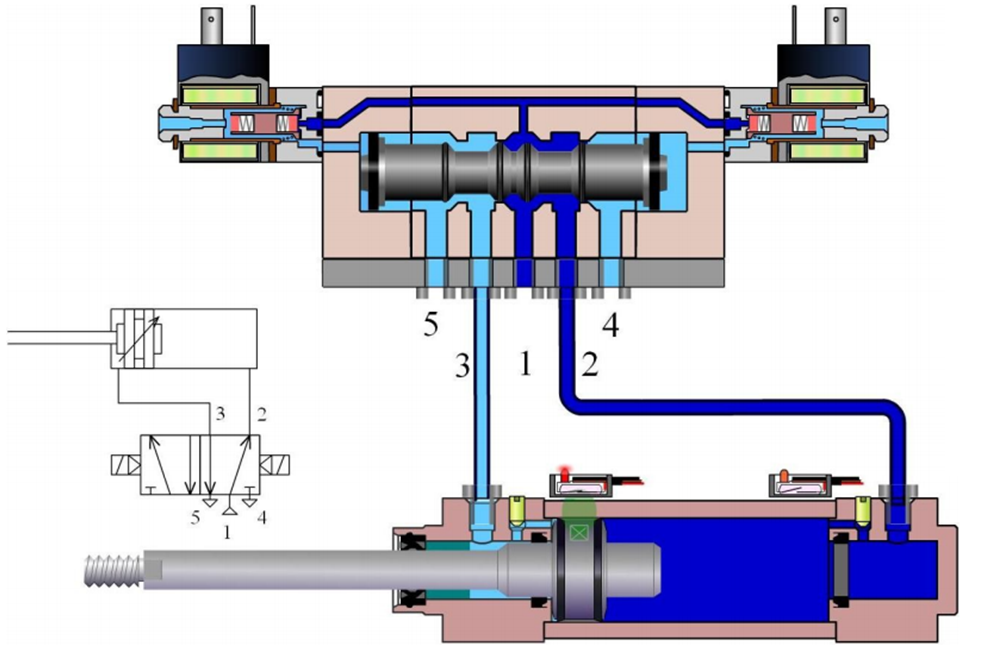
\includegraphics[width=5in]{media/image114.png}

\emph{Vérin double effet à amortissement réglable et distributeur 5/2
bistable à commande électropneumatique} 
\end{center}


\subsection{Désignation des distributeurs}

Lors de l'élaboration des schémas, il n'est pas possible de représenter
le distributeur, ainsi que les autres composants, sous leurs formes
commerciales. De ce fait, l'utilisation de symboles normalisés simplifie
la lecture et la compréhension des systèmes. Cette représentation
utilise la symbolisation par cases.

Un distributeur se représente sur les côtés droit et/ou gauche (comme
dans la réalité) par des pilotages. Ils permettent au tiroir de se
déplacer afin de mettre en communication les différents orifices.



\begin{defi}{Désignation}

La désignation d'un distributeur permet de mettre en évidence le nombre
d'orifices du distributeur, le nombre de positions, le type de commande
et son état (monostable ou bistable). 
\end{defi}

\begin{center}

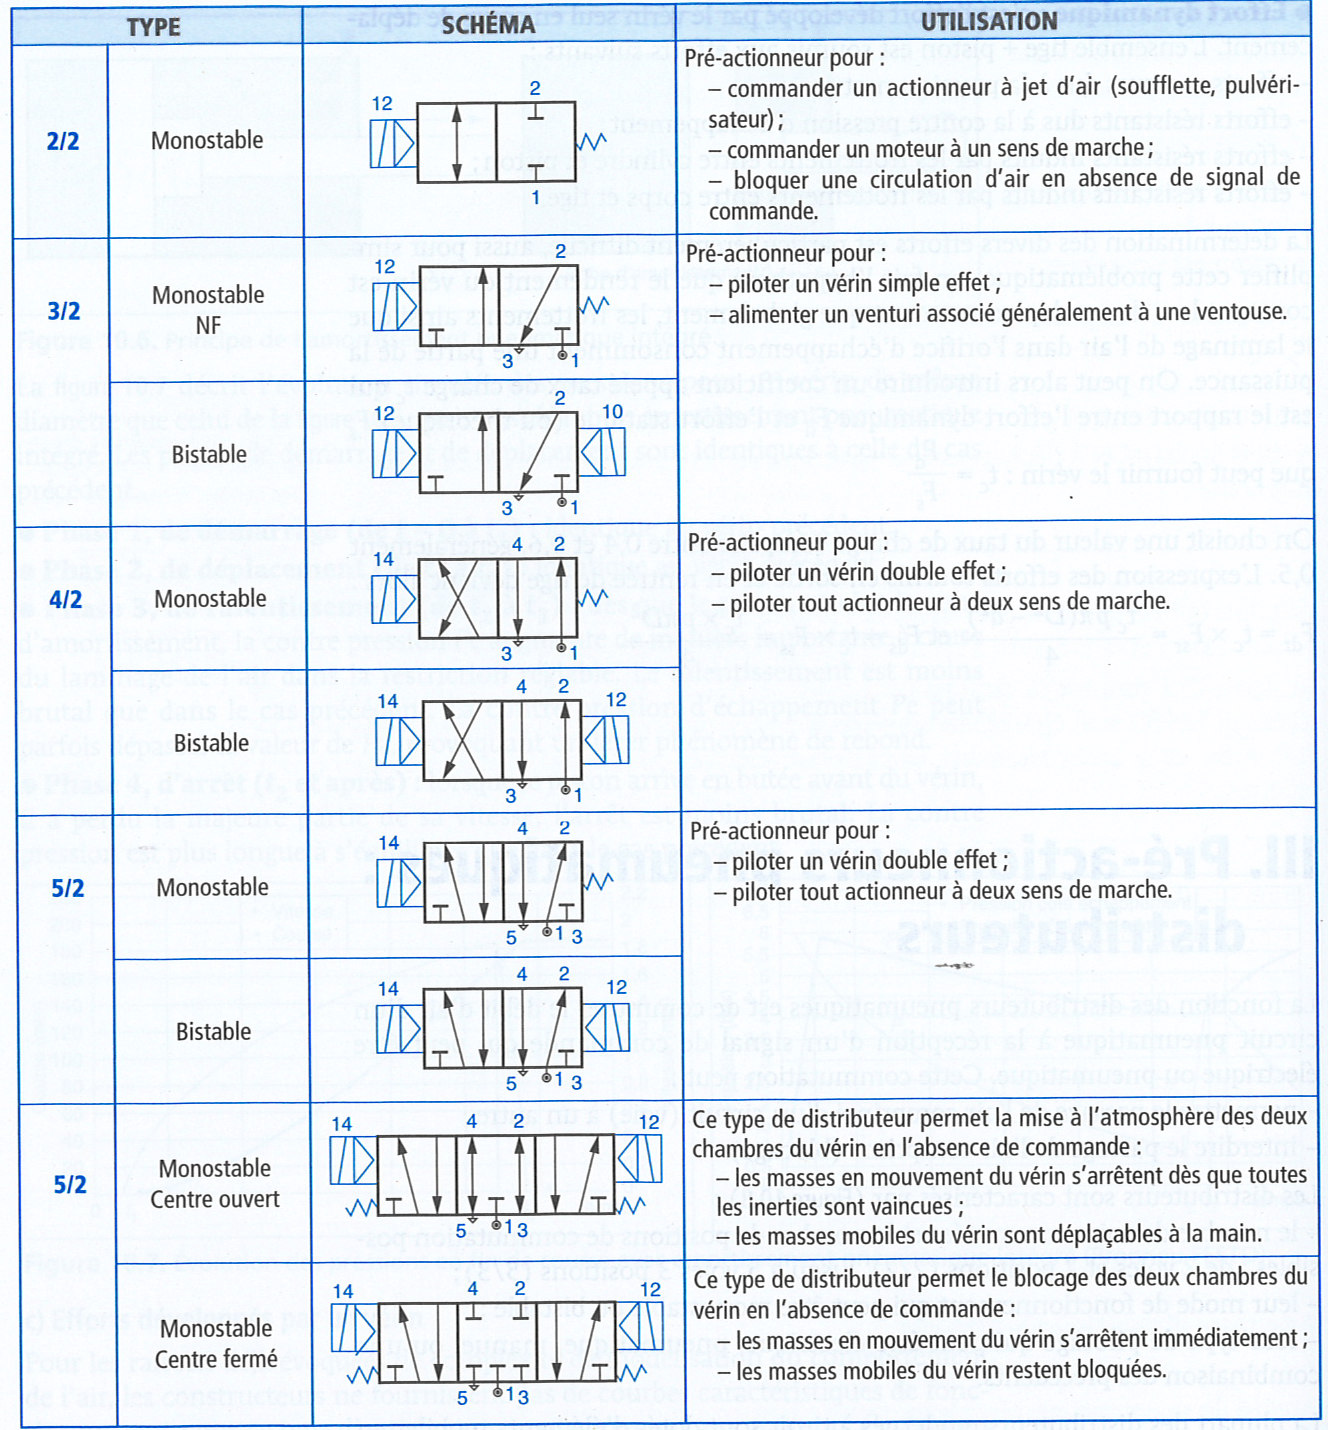
\includegraphics[width=5.5in]{media/image115.png}

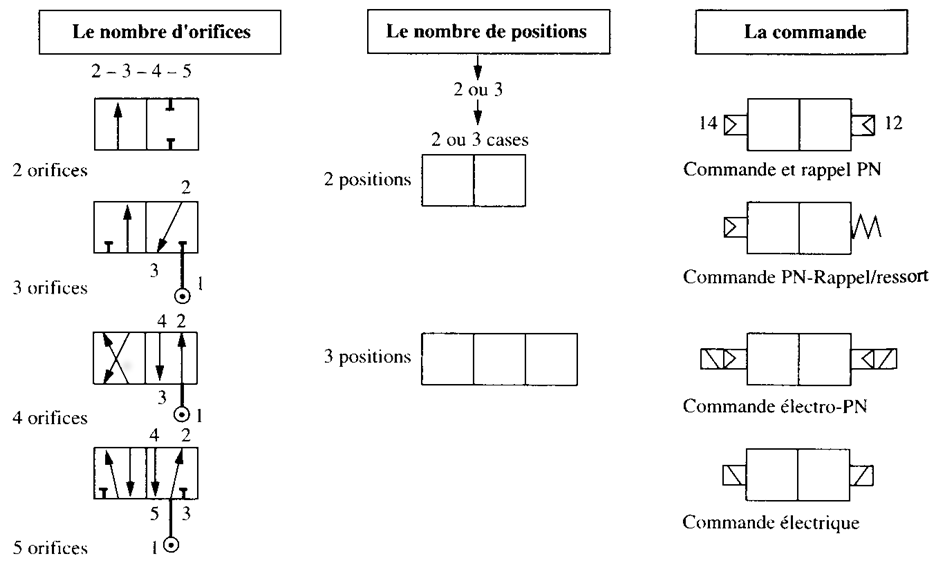
\includegraphics[width=5.5in]{media/image116.png}

\end{center}